\documentclass{beamer}

\usepackage{graphicx}
\usepackage{amsmath}
\usepackage{verbatim}
\usepackage{relsize}
\usepackage{listings}

\usetheme{Madrid}
\usecolortheme{wolverine}
\setbeamertemplate{navigation symbols}{}




\title{Effects of Injection Wells on Seismic Activity }
\author{W. Keil \& W. Cranford}
\institute{}





\begin{document}



\maketitle

\frame{\frametitle{Changepoint Analysis}
\textbf{Uses:} Used to detect significance changes in the mean or variance of data. 
\newline
\textbf{Method:}  Involves bootstrapping cumulative sum charts to detect change in mean or variance.
\newline
\textbf{Strengths}  Changepoint analysis can detect significant changes in means or variances when they are not apparent or they are hard to detect by other methods.  
\newline
\textbf{Results:} Changepoint analysis detected change in the mean of the total number of quakes per month at months: 173 184 218 225 232 
\newline
This translates to June 2010, May 2011, March 2014, October 2014, and May 1 2015. 
}



\frame{\frametitle{Changepoint Analysis}
\begin{center}
\includegraphics[scale=.115]{changepoint.png}
\end{center}
}

\frame{\frametitle{Total Earthquakes per Month, 1996 - 2015}
\begin{center}
\includegraphics[scale=.115]{quaketot.png}
\end{center}
}

\frame{\frametitle{Arima Model}
\textbf{Model:} Three parts: AutoRegressive(p) Differences(d) MovingAverage(q). 
\vspace{1.5mm}
\newline 
\(AR(p) = y_{t} = c + \phi_{1}y_{t-1} + \phi_{2}y_{t-2} + \dots + \phi_{p}y_{t-p} + e_{t} \) 
\vspace{2mm}
\newline 
Used \(8^{th} \) degree auto regressive function 
\vspace{2mm}
\newline 
\(2^{nd}\) degree differencing  \hspace{10mm} Zero order for Moving Average
\vspace{2mm}
\newline
AIC=1894.99   AICc=1896.55   BIC=1935.33
\vspace{2mm}
\newline
\(\phi_1 = -.7843\), \(\phi_2 =-.8428 \), \(\phi_ 3=-1.0816\), \(\phi_4 =-.4525 \)
\vspace{2mm}
\newline
\(\phi_5 =-.4248\), \(\phi_6=-.4053 \), \(\phi_ 7=-.0802 \), \(\phi_8 =-.0802 \)
}

\frame{\frametitle{Arima Forecast Results}
\begin{center}
\includegraphics[scale=.4]{arimaplot.png}
\end{center}
}


\frame{\frametitle{Number of Earthquakes Over Time}
\begin{center}
\includegraphics[scale=.55]{earthtime_mag.png}
\end{center}
}

\frame{\frametitle{Magnitude of Earthquakes Over Time}
\textbf{December 1974 - January 2008:}
\newline
 Average of \( 1.96\) Earthquakes \( > 2.5 \) magnitude per year. 
\newline
Average magnitude of all earthquakes in this period is \(2.51\). 
\newline

\textbf{February 2008 - September 2016:} 
\newline
 Average of \( 623.3\) Earthquakes \( > 2.5 \) magnitude per year. 
\newline
Average magnitude of all earthquakes in this period is \(2.74\). 
}

\frame{\frametitle{Total BBLS vs MAG for 5 Mile Radius}
\begin{center}
\includegraphics[scale=.55]{bbls_mag_5.png}
\end{center}
}


\frame{\frametitle{Total BBLS vs MAG for 10 Mile Radius}
\begin{center}
\includegraphics[scale=.55]{bbls_mag_10.png}
\end{center}
}


\frame{\frametitle{Total BBLS vs MAG for 15 Mile Radius}
\begin{center}
\includegraphics[scale=.55]{bbls_mag_15.png}
\end{center}
}

\frame{\frametitle{Model Results}
\textbf{Linear Model Relations}
\newline
Evidence of nonzero correlation between bbls and magnitude. \newline
\vspace{10mm}
\newline
\textbf{Random Forest Predictions}  \newline
Able to predict magnitude with good accuracy. 

}

\frame{\frametitle{Significance of Results}
\textbf{Injection Activity Regulation}
\newline

}

\frame{\frametitle{Locational Data Sets}
\textbf{Objective:}
\newline Try to predict the locations of earthquakes with magnitude of 2.5 or higher. 
\newline

\textbf{Data:} 
\newline Twenty data-frames, each one representing one year of data. 
\newline The columns contain all relevant drilling and seismic information.
\newline Each row represents a different location in Oklahoma. 
}


\frame{\frametitle{Overview of Location Data Sets}
\begin{center}
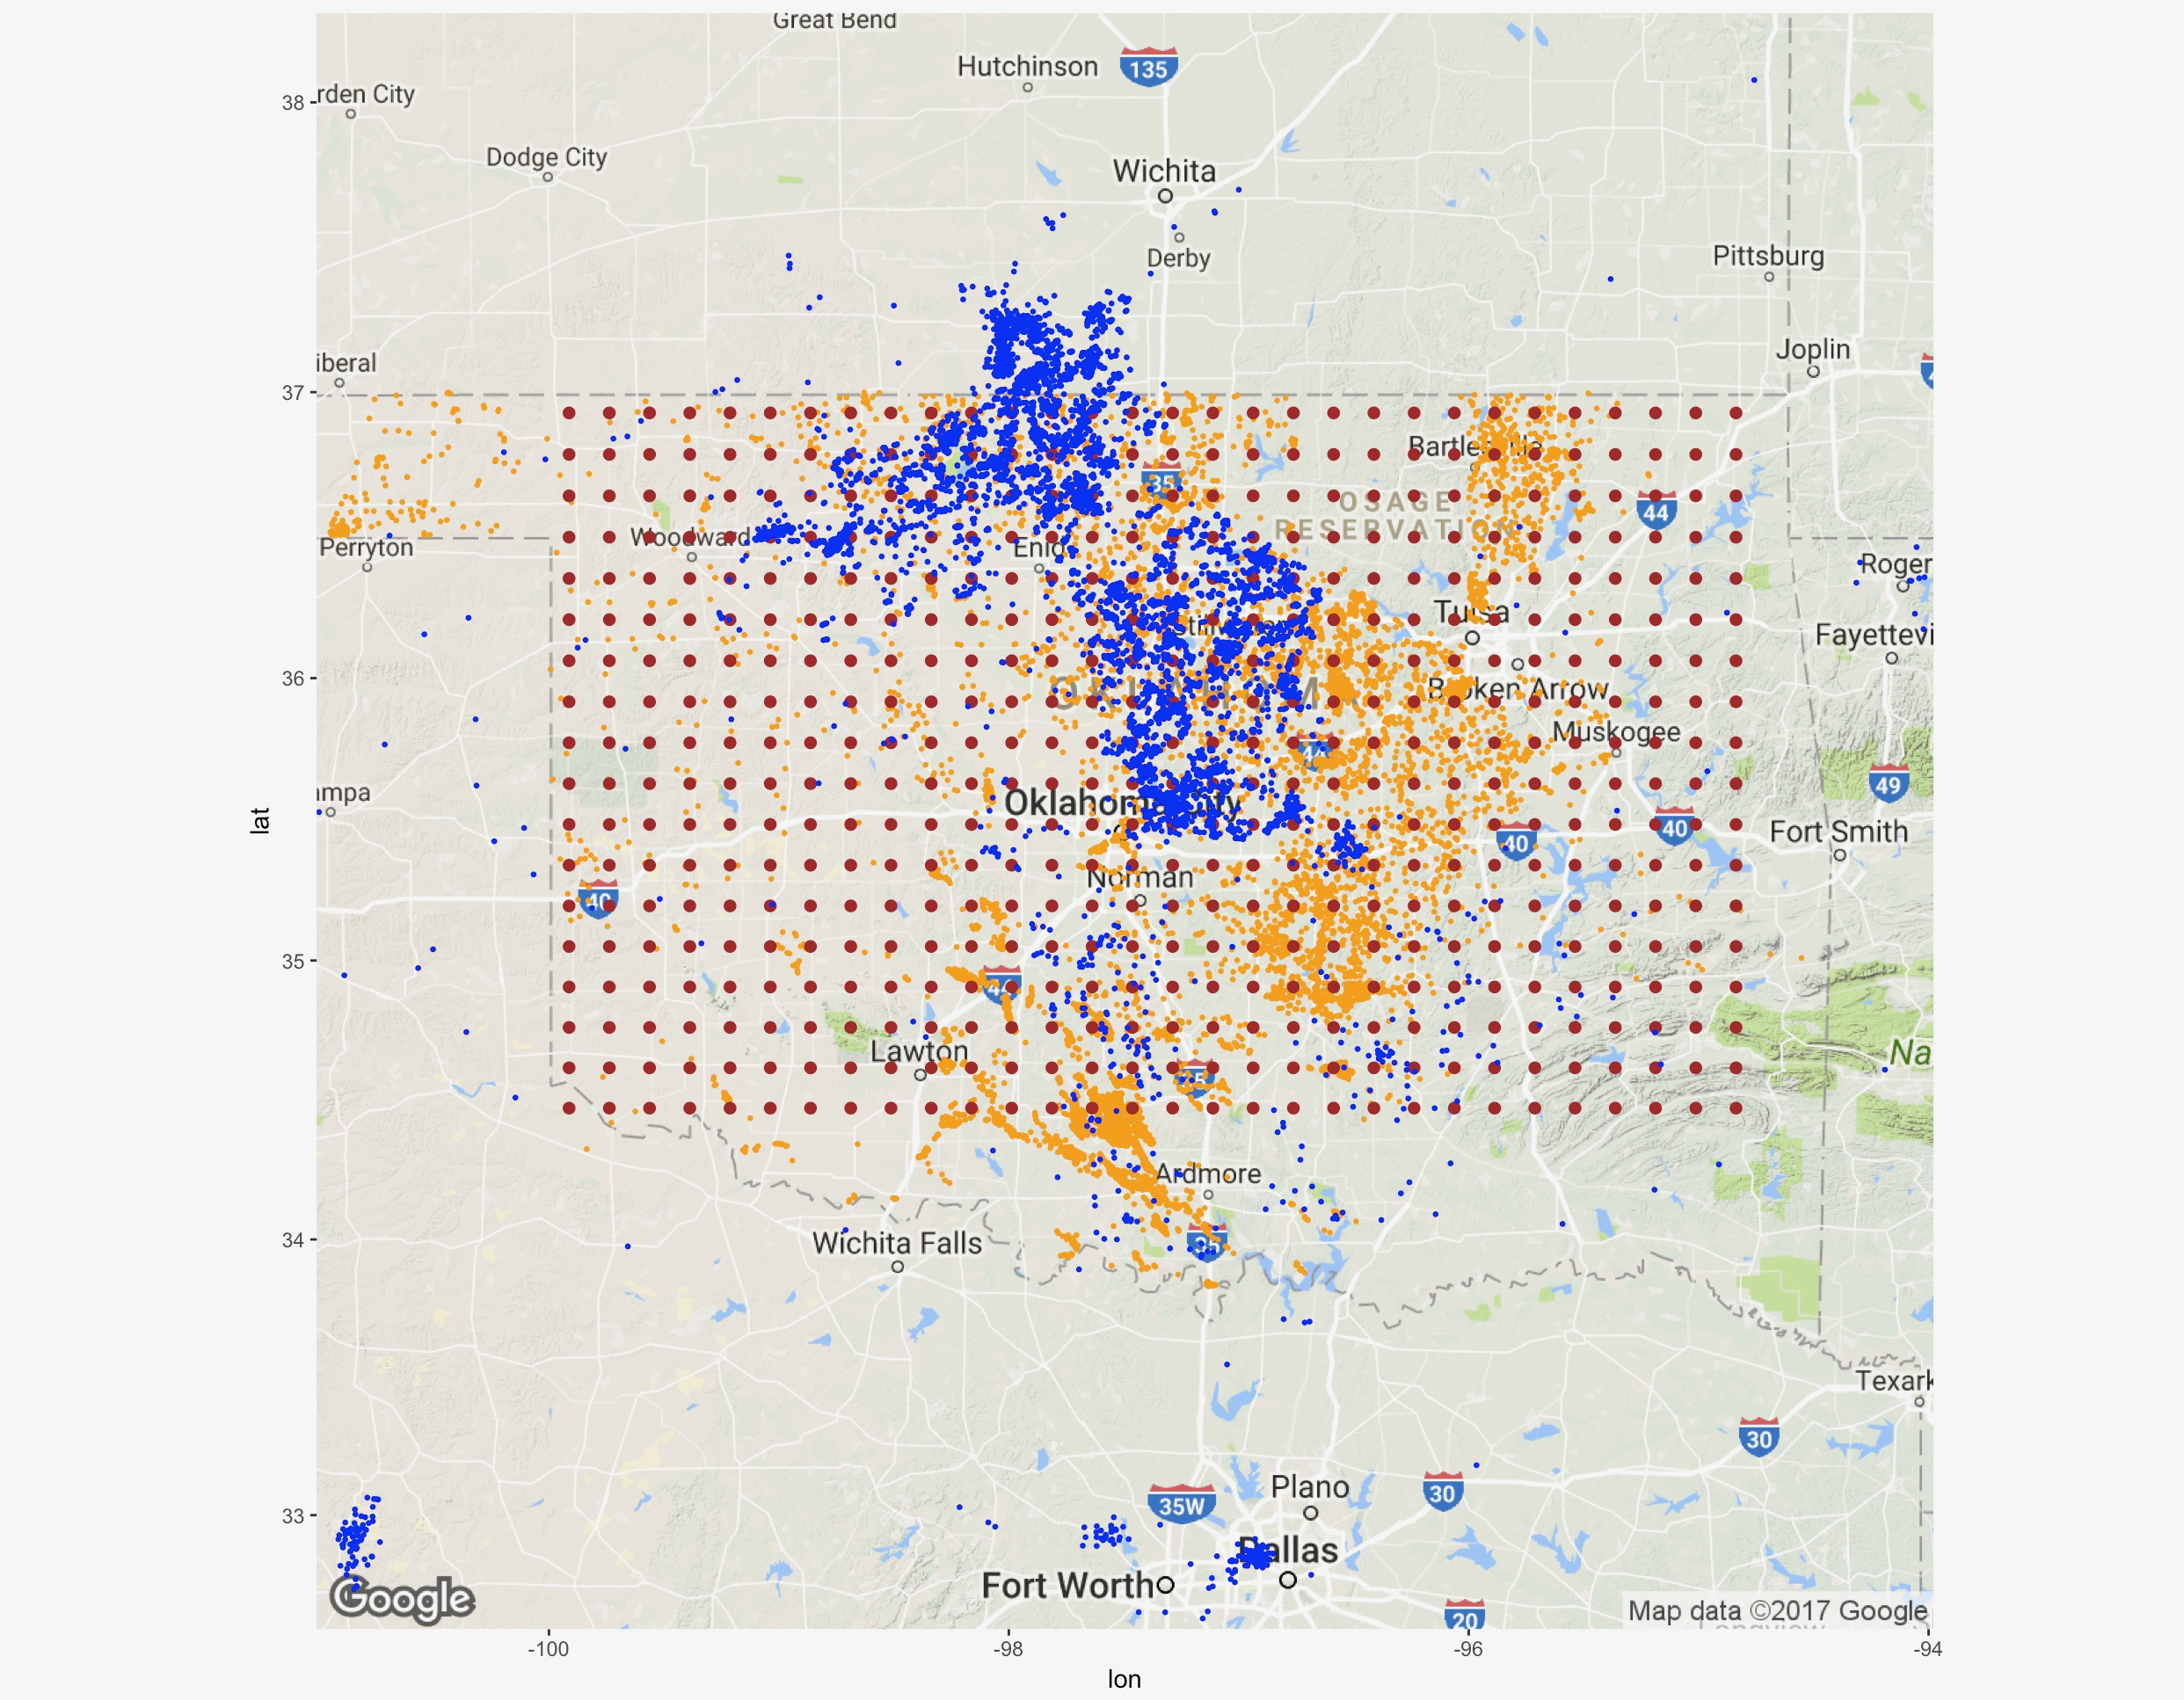
\includegraphics[scale=.115]{data540.png}
\end{center}
}


\frame{\frametitle{Meta Ensembling}
\textbf{Model:}
\newline Meta Ensembling - a.k.a.  Model Stacking. 
\newline A well establish technique.
\newline Involves running multiple different models and using the results as inputs for a different model. 

\textbf{Motivation:} 
\newline Originally ran random forest model with interesting but uninterpretable results. 
\newline Decided to take the prediction values of a random forest model and use them in inputs for a SVM model. 
}


\frame{\frametitle{SVM Stacked Model}
Tune ( svm, catbigquake - rfpred, numwells, sumbbls  ) 
\vspace{10mm}
\newline
\textbf{catbigquake} - The categorical variable of whether a location will have at least one 2.5 magnitude earthquake in a given year. 
\newline
\textbf{rfpred} - The prediction result of random forest model trying to predict the average magnitude of earthquakes in each location. 
\newline
\textbf{numwells} - The number of wells drill per location in a given year. 
\newline
\textbf{sumbbls} - The sum of the number of barrels of fluids pumped into the ground per year. 

}

\frame{\frametitle{SVM 2013 - Error Rate 11.48 \%}
\begin{center}
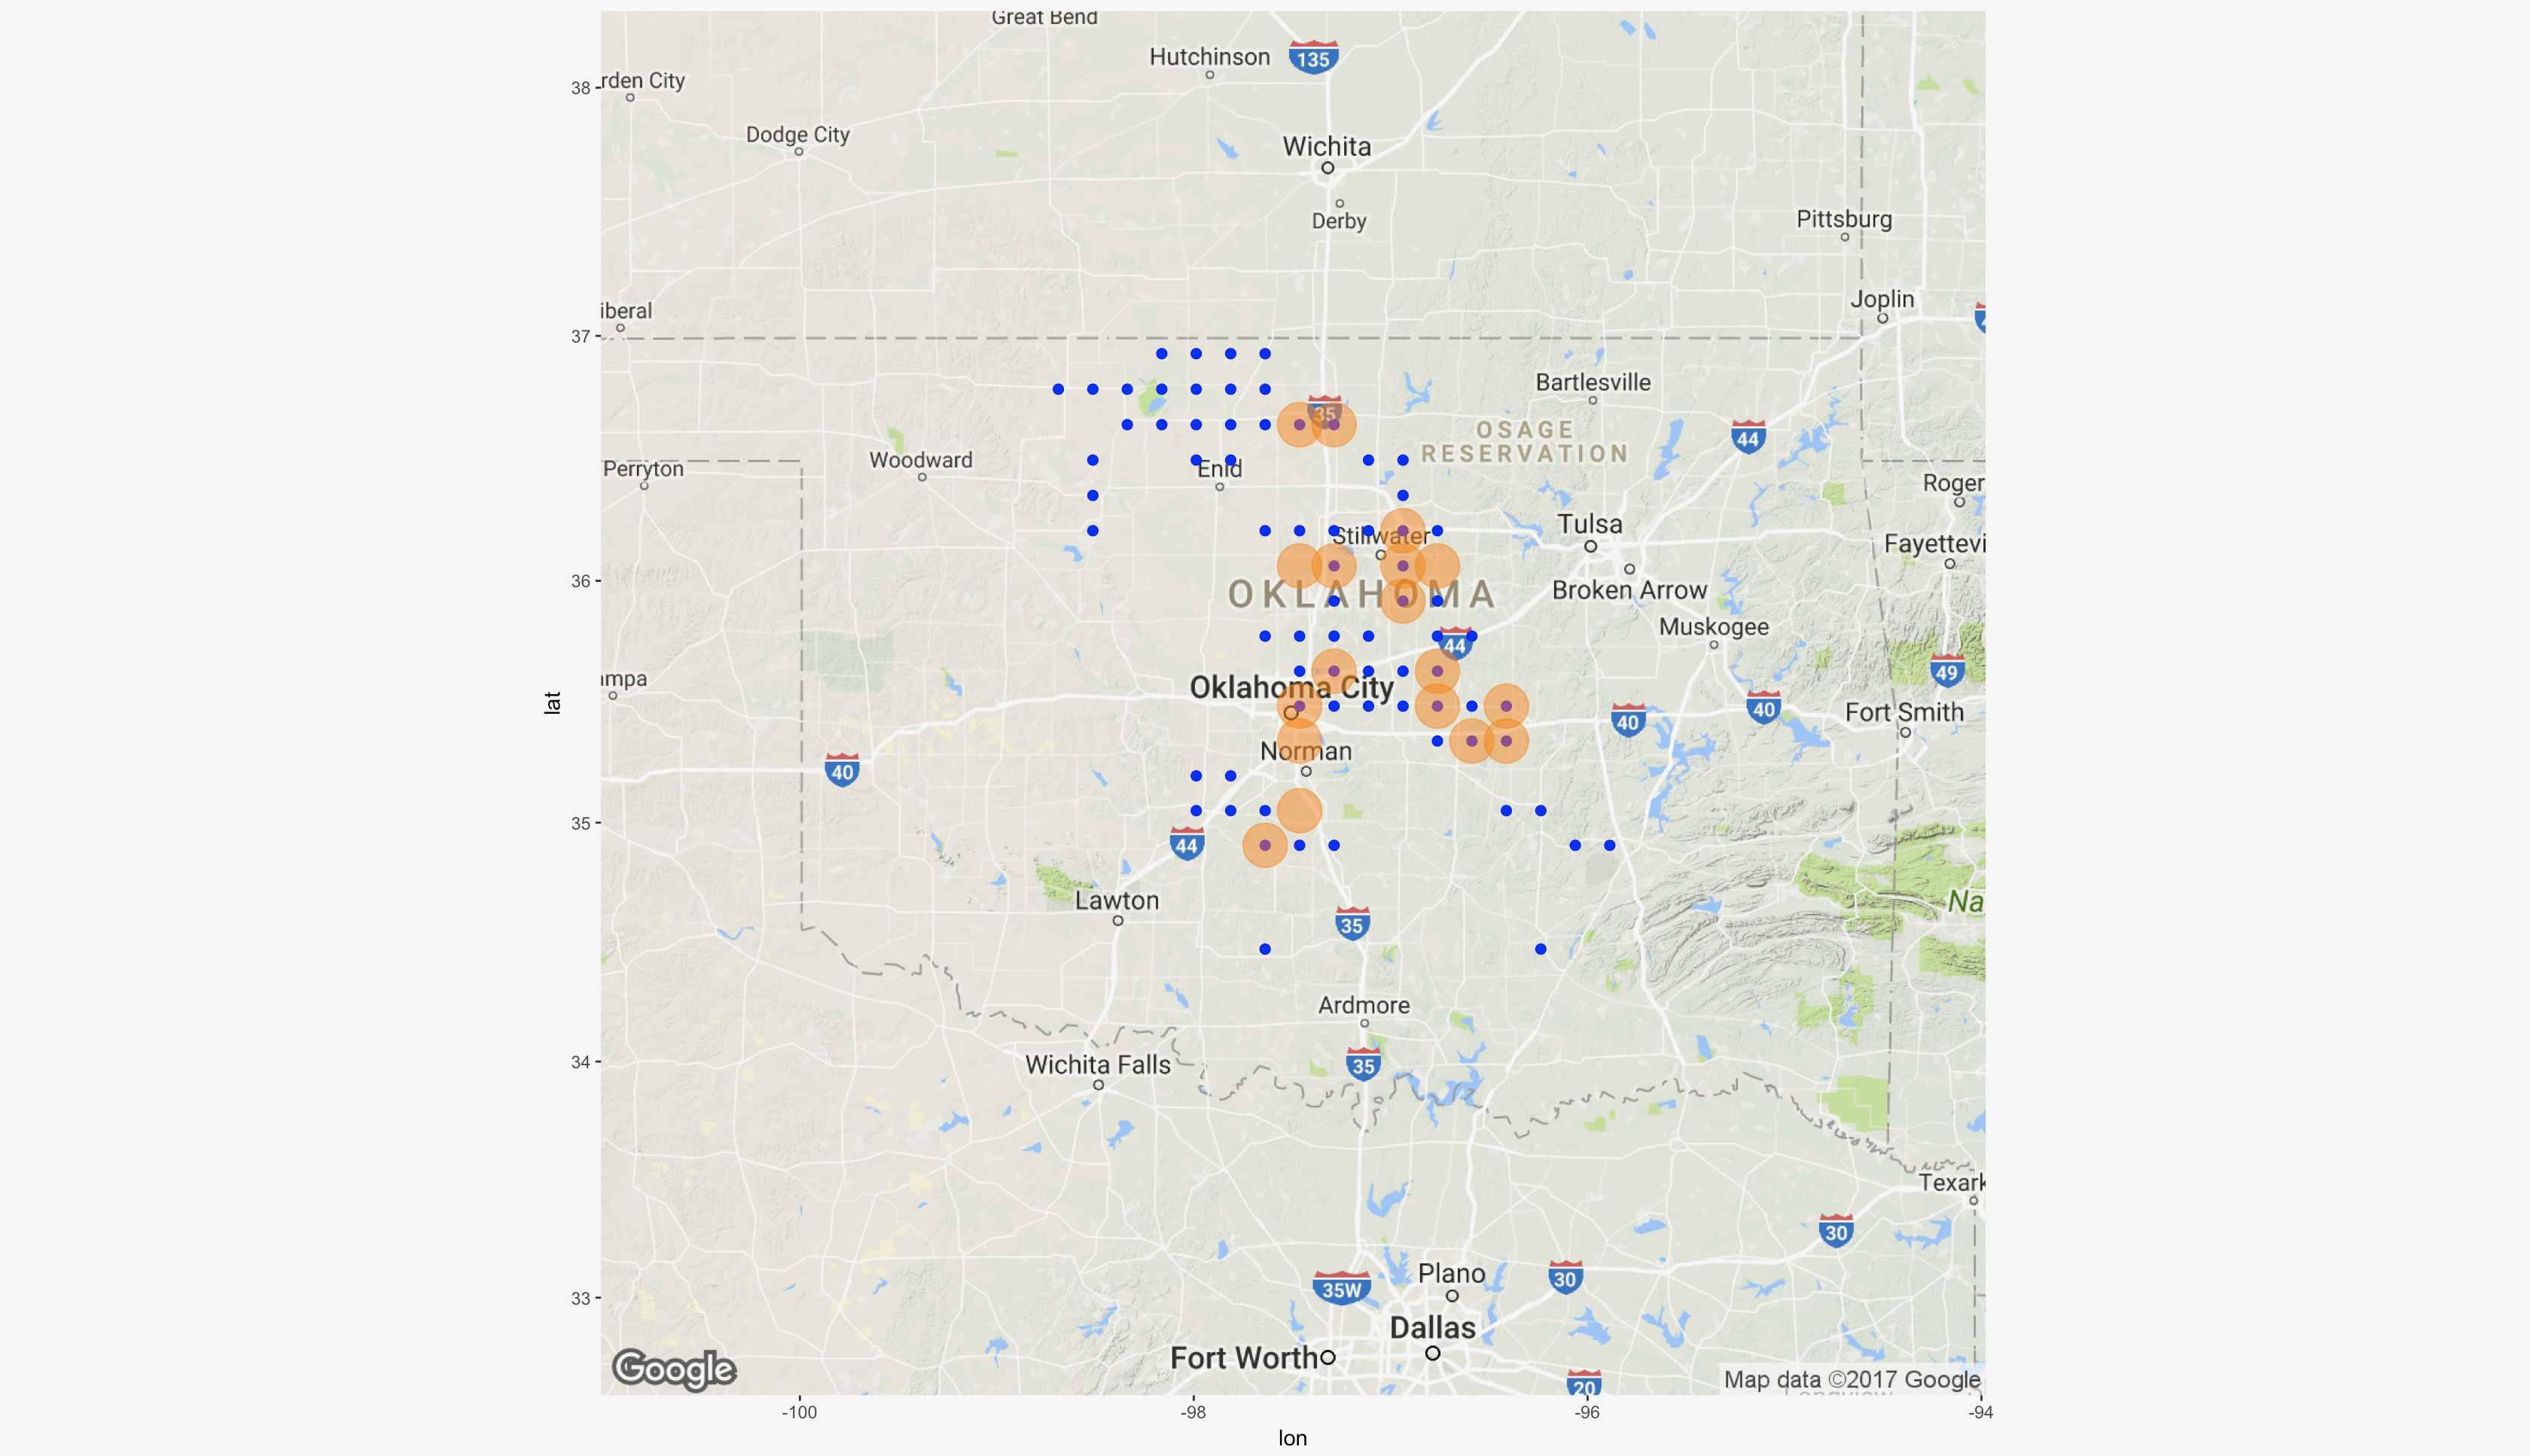
\includegraphics[scale=.115]{svmpred13.png}
\end{center}
}


\frame{\frametitle{SVM 2014 - Error Rate 15.19 \%}
\begin{center}
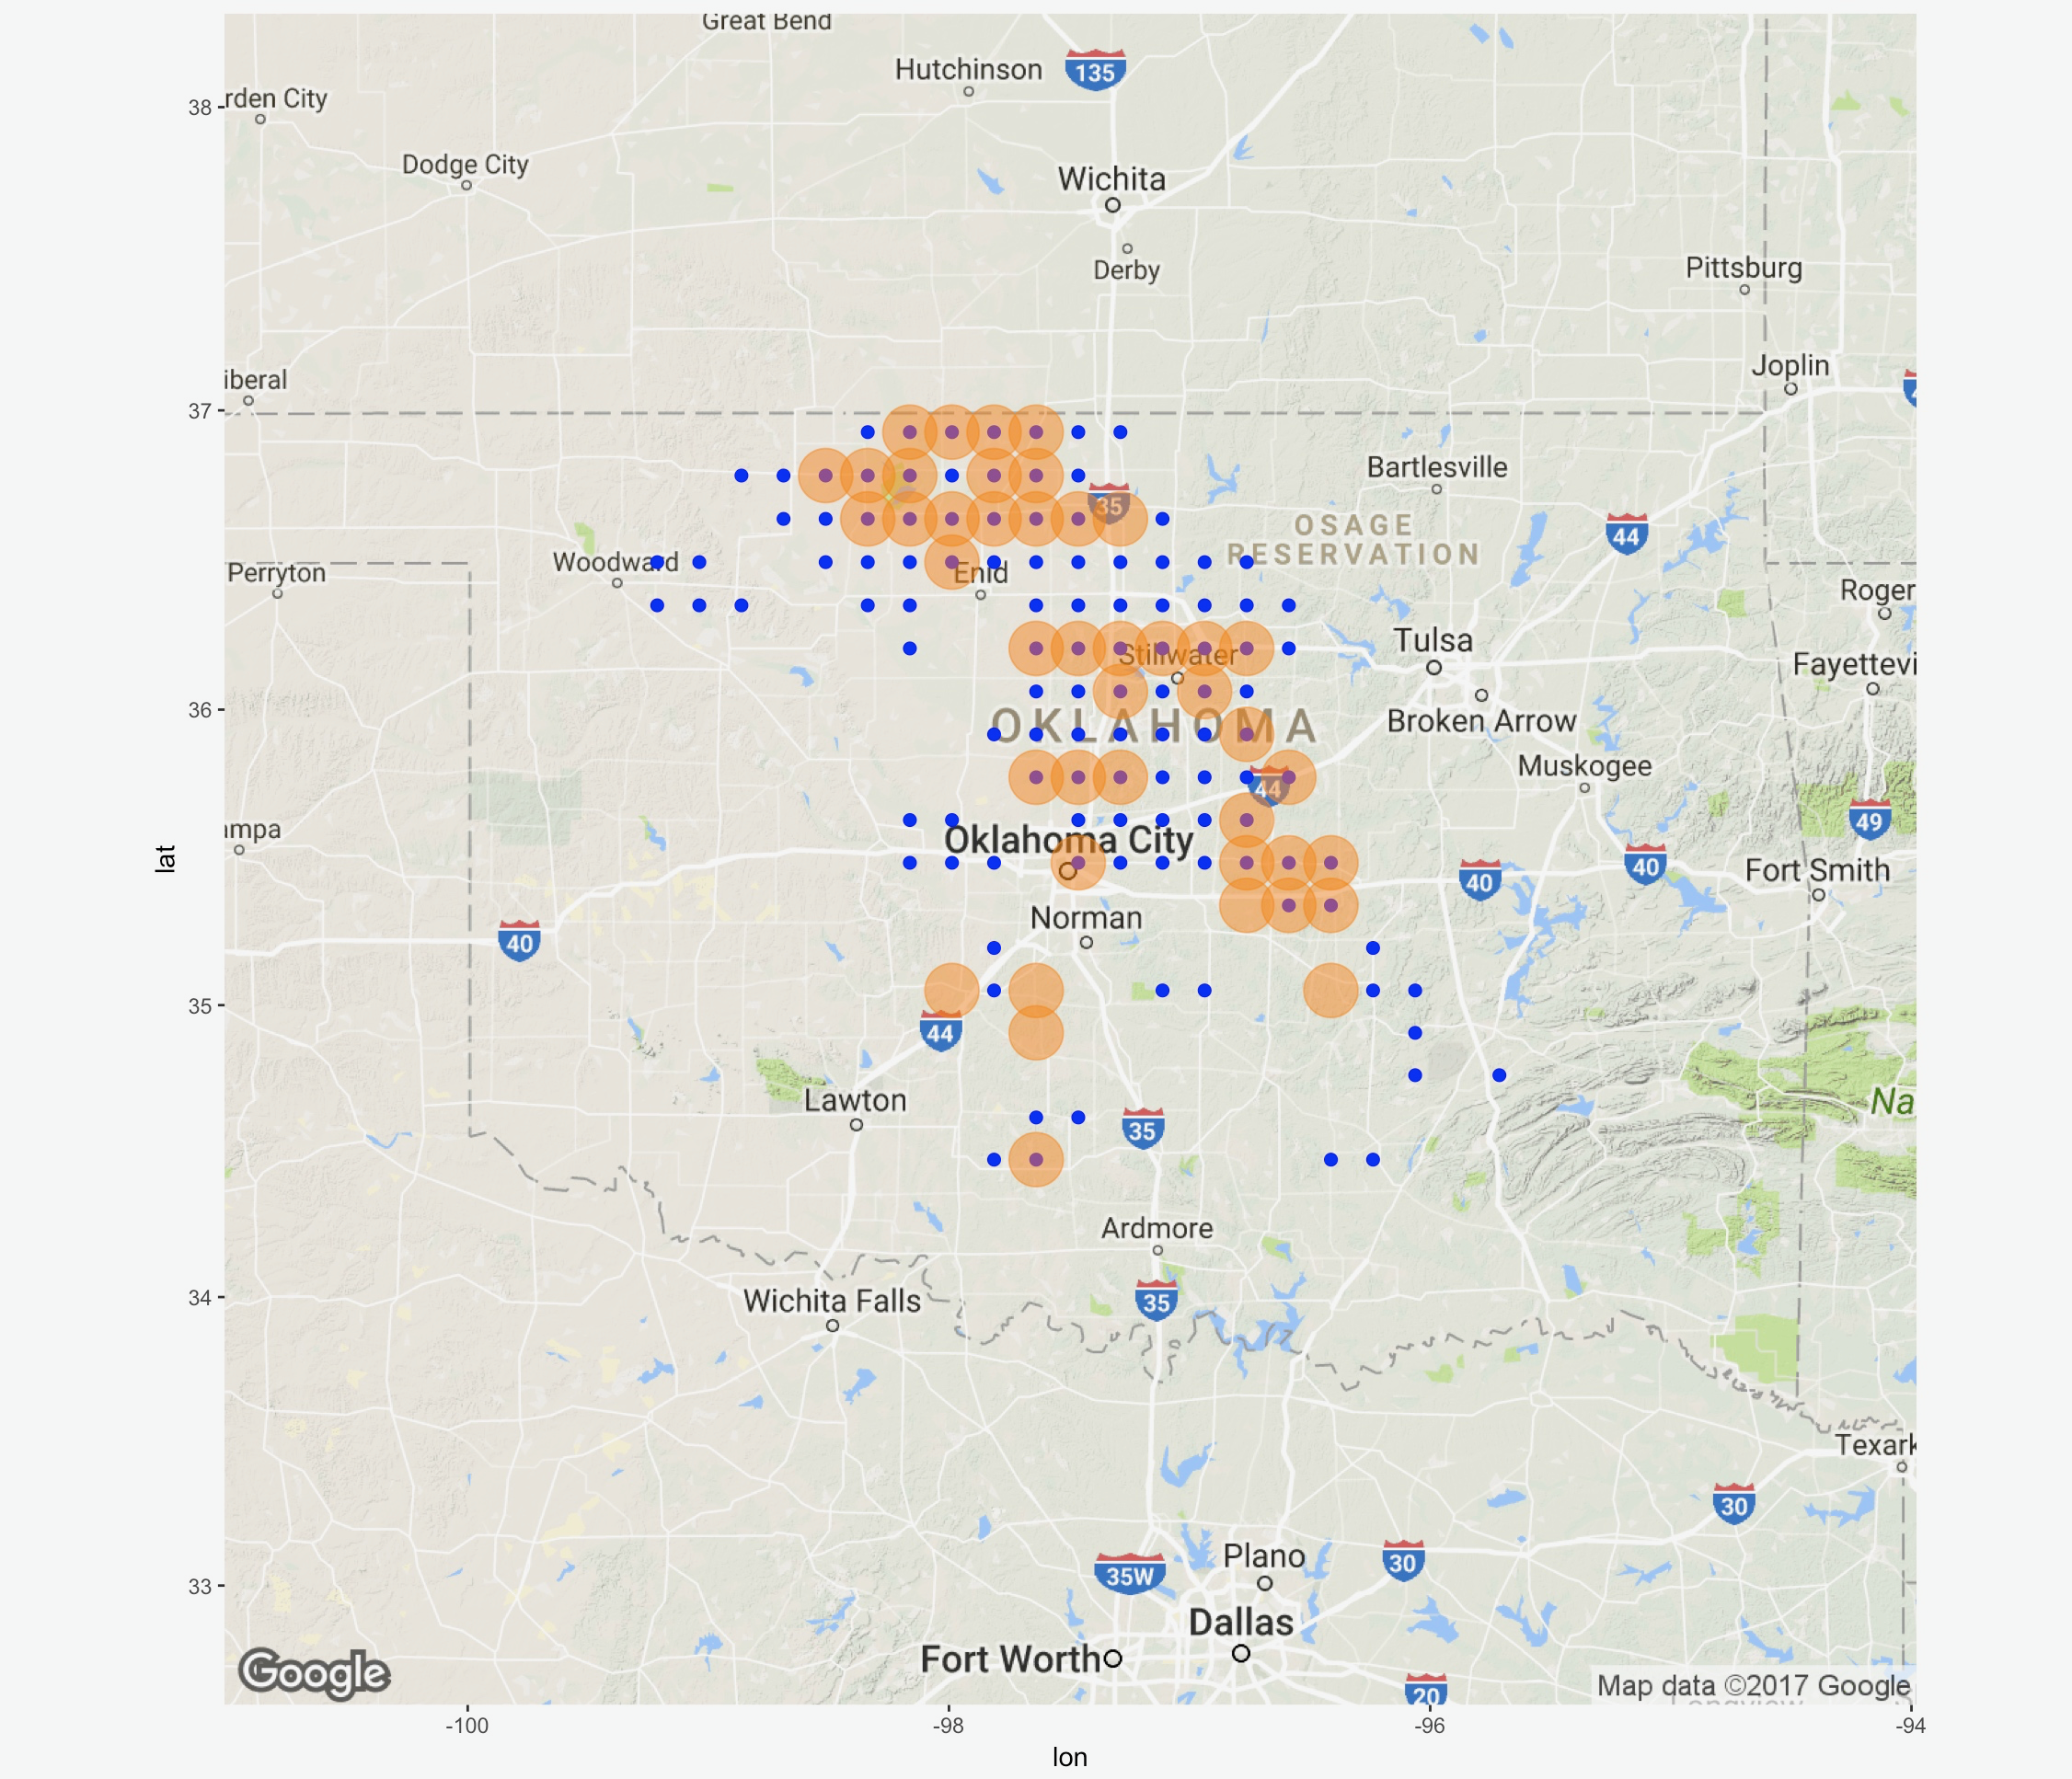
\includegraphics[scale=.115]{2014_svm.png}
\end{center}
}


\frame{\frametitle{SVM 2015 - Error Rate 14.07 \%}
\begin{center}
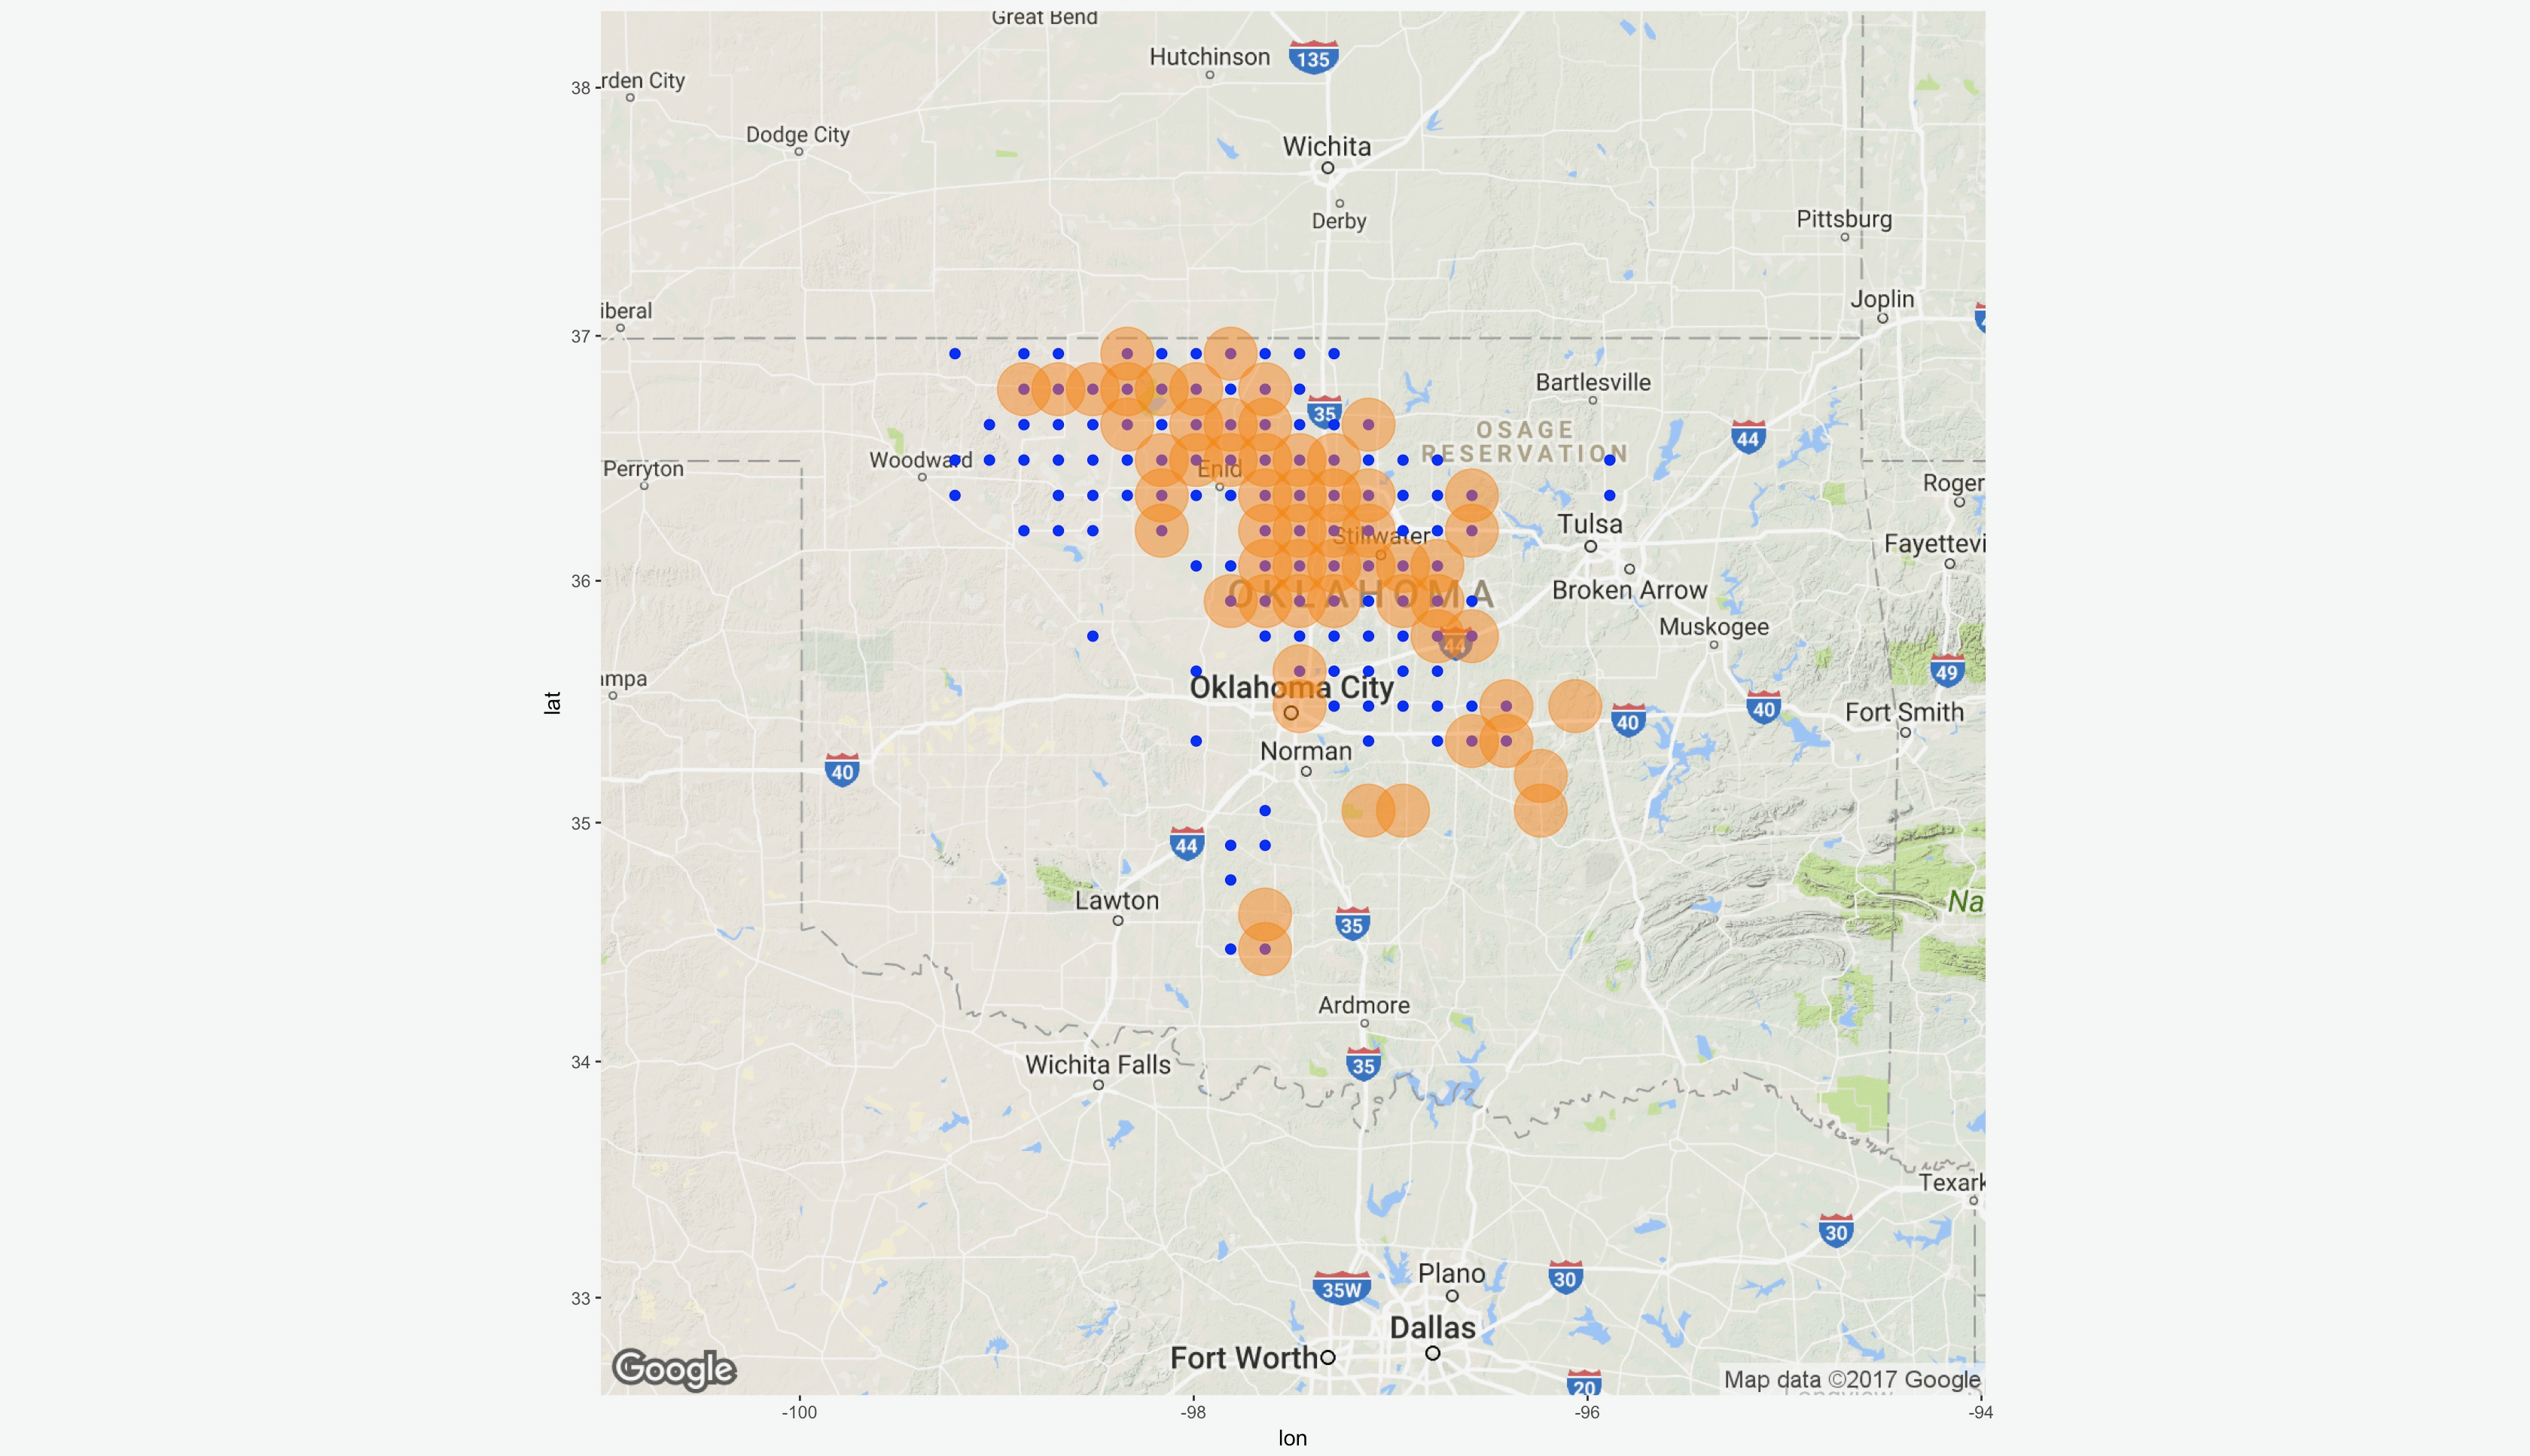
\includegraphics[scale=.115]{svmpred15.png}
\end{center}
}



\frame{\frametitle{SVM Results- Confusion Matrices }
\hspace{38mm}    2013  \hspace{7 mm}    2014   \hspace{7mm} 2015 
\[
\begin{bmatrix}
  464 &  58 \\
  4  & 14
\end{bmatrix}  
\begin{bmatrix}
  421 & 76  \\
   6 & 37
\end{bmatrix}
\begin{bmatrix}
    413&  69  \\
     7 & 51
\end{bmatrix}
\]
\hspace{5mm} Error Rates  \hspace{7 mm} 11.48 \%  \hspace{7 mm} 15.19 \%   \hspace{3mm} 14.07 \% 
}



\end{document}












